%compile with pdflatex on papeeria

\documentclass[a4paper,12pt]{article}
\usepackage{fancyhdr}
%\usepackage{fancyheadings}
\usepackage[ngerman,german]{babel}
\usepackage{german}
\usepackage[utf8]{inputenc}
%\usepackage[latin1]{inputenc}
\usepackage[active]{srcltx}
%\usepackage{algorithm}
%\usepackage[noend]{algorithmic}
\usepackage{amsmath}
\usepackage{amssymb}
\usepackage{amsthm}
\usepackage{bbm}
\usepackage{enumerate}
\usepackage{graphicx}
\usepackage{ifthen}
\usepackage{listings}
\usepackage{enumitem}
%\usepackage{struktex}
\usepackage{hyperref}
\usepackage{tikz}
\usepackage{float}
\usepackage{subcaption}
\usepackage{array}
\captionsetup{compatibility=false}
\captionsetup[subfigure]{labelformat=empty}

\usepackage{pgfplots}
\usepgfplotslibrary{fillbetween}
%\usetikzlibrary{patterns}
\pgfplotsset{compat=1.15}
\usepackage{mathrsfs}
\usetikzlibrary{arrows}

\pgfplotsset{grid style={dashed,gray}}

\definecolor{kolorwykresu}{rgb}{0.07,0.04,0.56}

\pagenumbering{gobble}

\usepackage{tabularray}
\usepackage{multirow}
\usepackage{booktabs,tabularx}
\renewcommand\tabularxcolumn[1]{m{#1}}% for vertical centering text in X column

\newcolumntype{L}[1]{>{\raggedright\let\newline\\\arraybackslash\hspace{0pt}}m{#1}}
\newcolumntype{C}[1]{>{\centering\let\newline\\\arraybackslash\hspace{0pt}}m{#1}}
\newcolumntype{R}[1]{>{\raggedleft\let\newline\\\arraybackslash\hspace{0pt}}m{#1}}

\newcolumntype{Y}{>{\centering\arraybackslash}X}

%%%%%%%%%%%%%%%%%%%%%%%%%%%%%%%%%%%%%%%%%%%%%%%%%%%%%%
%%%%%%%%%%%%%% EDIT THIS PART %%%%%%%%%%%%%%%%%%%%%%%%
%%%%%%%%%%%%%%%%%%%%%%%%%%%%%%%%%%%%%%%%%%%%%%%%%%%%%%
\newcommand{\Fach}{1. Klausur aus der Mathematik (A)}
\newcommand{\Name}{}
\newcommand{\datum}{}
\newcommand{\Matrikelnummer}{}
\newcommand{\Semester}{Q12/1}
\newcommand{\Uebungsblatt}{} %  <-- UPDATE ME
%%%%%%%%%%%%%%%%%%%%%%%%%%%%%%%%%%%%%%%%%%%%%%%%%%%%%%
%%%%%%%%%%%%%%%%%%%%%%%%%%%%%%%%%%%%%%%%%%%%%%%%%%%%%%

\setlength{\parindent}{0em}
%\topmargin -1.0cm
\oddsidemargin 0cm
\evensidemargin 0cm
\setlength{\textheight}{9.2in}
\setlength{\textwidth}{6.0in}

%%%%%%%%%%%%%%%
%% Aufgaben-COMMAND
\newcommand{\Aufgabe}[1]{
  {
  \vspace*{0.5cm}
  \textsf{\textbf{Aufgabe #1}}
  \vspace*{0.2cm}
  
  }
}
%%%%%%%%%%%%%%
\hypersetup{
    pdftitle={\Fach{}: Übungsblatt \Uebungsblatt{}},
    pdfauthor={\Name},
    pdfborder={0 0 0}
}

\lstset{ %
language=java,
basicstyle=\footnotesize\tt,
showtabs=false,
tabsize=2,
captionpos=b,
breaklines=true,
extendedchars=true,
showstringspaces=false,
flexiblecolumns=true,
}

\title{Übungsblatt \Uebungsblatt{}}
\author{\Name{}}

\begin{document}

\fancyhead{}
\fancyhead[C]{
\includegraphics[height=2.5cm]{lukasLogo.png}
\vspace{2cm}
}

\thispagestyle{fancy}
%\lhead{\sf \large \Fach{} \\ %\small \Name{} - \Matrikelnummer{}


\lhead{
%\vspace{1cm}
  \sf \LARGE \Fach{} %\small \Name{} - \Matrikelnummer{}
}
\rhead{\sf \Semester{}   \datum{}}

\vspace*{0.2cm}

\vspace{4cm}
Alle Lösungen müssen mit Nebenrechnungen und Begründungen nachvollziehbar sein!

%\rhead{\sf \Semester{} }
\vspace*{0.2cm}
%\begin{center}
%%\LARGE \sf \textbf{Übungsblatt \Uebungsblatt{}}
%\end{center}
%\vspace*{0.2cm}

%%%%%%%%%%%%%%%%%%%%%%%%%%%%%%%%%%%%%%%%%%%%%%%%%%%%%%
%% Insert your solutions here %%%%%%%%%%%%%%%%%%%%%%%%
%%%%%%%%%%%%%%%%%%%%%%%%%%%%%%%%%%%%%%%%%%%%%%%%%%%%%%

\vspace{1cm}
  Name: \underline{\hspace{7cm}}
%\draw[line width=1pt,color=ccqqqq,smooth,samples=100,domain=-6:7] plot(\x,{(1/12)*\x*\x+(1/3)*\x});
  \hfill
  Datum: \underline{\hspace{4cm}}

%\vspace{0,5cm}Die Rechenwege müssen nachvollziehbar sein!

%\vspace{1,5cm} {TEIL A} - ohne Hilfsmittel. Bearbeitungszeit 35 min.
\vspace {2cm}


\begin{center}
  \begin{tblr}{
      width=1\linewidth,
      colspec = {Q[c,6em]Q[c,4em]Q[c,4em]Q[c,4em]Q[c,4em]Q[c,4em]Q[c,4em]Q[c,6em]},
      rowspec = {Q[m]Q[m]Q[m]Q[m]Q[m]Q[m]Q[m]Q[m]},
      colsep = 0mm,
      %row{1} = {2em,azure2,fg=white,font=\large\bfseries\sffamily},
      row{1} = {2em,font=\large\bfseries\sffamily},
      hlines, vlines,
    }
    \textbf{Aufgabe} & \textbf{1} & \textbf{2} & \textbf{3} & 
    \textbf{4} & \textbf{5} & \textbf{6} & \textbf{Gesamt} \\
    {Mögliche \\ Punkte} & {6} & {8} & {6} & 5 & 7 & 10 & 42 \\
    {Erreichte \\ Punkte} &  &  &  &  &  &  &  \\
  \end{tblr}
\end{center}

\vspace{5cm}
\centerline{\huge\bfseries\sffamily Viel Erfolg !!!}

\newpage

\Aufgabe{1: (3BE+3BE)} 
Gegeben ist der Graph der Funktion $f$. 
\begin{enumerate}[label={\alph*)}] 
  \item Bestimmen Sie näherungsweise den Wert des Integrals ${\int_{0}^{10} f(x)\, dx}$ und ermitteln Sie die prozentuale Abweichung von dem realen Wert von 51.
\begin{figure}[H]
  \centering
  \includegraphics[width=1\columnwidth]{211117_8.png}
  %\caption{A boat.}
  %\label{fig:boat1}
\end{figure}
\newpage
  \item Gegeben ist der Graph der Funktion $f$ aus Teilaufgabe a). Skizzieren Sie einen möglichen Verlauf der Ableitungs- und Stammfunktion von $f$ in das gegebene Koordinatensystem.
\end{enumerate}
\begin{figure}[H]
  \centering
  \includegraphics[width=1\columnwidth]{211117_8.png}
  %\caption{A boat.}
  %\label{fig:boat1}
\end{figure}


\vspace{3cm}

\Aufgabe{2: (3BE+5BE)} 
\begin{enumerate}[label={\alph*)}] 
  \item Berechnen Sie den Wert des Integrals:
    \[ \int_{3}^{5} \frac{x+1}{2(0,5x^2+x)}\,dx \]
  \item Bestimmen Sie den Inhalt der Fläche, die die Graphen der Funktionen ${f(x)= \frac{1}{4}x^2}$ und ${g(x) = x+3}$ mit der $y$-Achse im 1. Quadranten einschließen. (Skizze!)
\end{enumerate}

\Aufgabe{3: (?BE)} 
Ein Antibiotikum wird in unterschiedlichen Wirkstoffkonzentrationen produziert. Den zeitlichen Verlauf der Wirkstoffkonzentration im Blut beschreibt ein Mathematiker durch folgende Funktionenschar:
\[f_k: t \rightarrow  k \cdot t \cdot e^{-0,2t} \quad  t\ge0 \quad k>0 \]

Es wird die Zeit $t$ in Stunden seit der Einnahme und die Wirkstoffkonzentration $f(t)$ im Blut in $\frac{mg}{l}$ gemessen.

\begin{enumerate}[label={\alph*)}]
  \item Bestimmen Sie $f_k(0)$ sowie $\lim \limits_{t \to \infty} f_k(t)$ und interpretieren Sie im Sachzusammenhang.
  \item Zeigen Sie, dass für den Term der Ableitungsfunktion von $f_k$, gilt: 
    \[g_k (t) = k \cdot e^{-0,2t} (1-0,2t) \]
  \item Bestimmen Sie rechnerisch Monotonie und Extremwerte der Funktionenschar $f_k$ nach Art und Lage. 
    Formulieren Sie nun den Einfluss des Parameters $k$ in Worten. Argumentieren Sie dabei unter Einbeziehung der Anwendungssituation.
  \item Die maximale Wirkstoffkonzentration im Blut soll $11\frac{mg}{l}$ betragen. Ermitteln Sie den zugehörigen Parameter $k$.
\end{enumerate}

Gerundetes Zwischenergebnis für die folgenden Aufgaben: 
\[ f(t)=6 \cdot t \cdot e^{-0,2t} \]


\begin{enumerate}[label={\alph*)}]
  \item Bestimmen Sie den Zeitpunkt, zu dem der Wirkstoff am stärksten abgebaut wird. Argumentieren Sie unter Verwendung der mathematischen Fachsprache und dokumentieren Sie Ihren Gedankengang ausführlich im Anwendungskontext.
  \item Skizzieren Sie den Graphen von $f$ ausschließlich unter Verwendung der bisherigen Ergebnisse im Bereich $0 \le t \le 24$.
\end{enumerate}

\newpage
\Aufgabe{4: (3BE+2BE)} 
\begin{enumerate}[label={\alph*)}] 
  \item Bestimmen Sie eine ganzrationale Funktion höchstens vierten Grades, deren Graph bzgl. der $y$-Achse symmetrisch ist und in $P (-1|1)$ eine Wendetangente mit der Steigung 3 hat.
  \item Geben Sie einen Funktionsterm einer Funktion $f$ an, dessen Graph streng monoton steigt und rechtsgekrümmt ist.
\end{enumerate}


%\Aufgabe{5: (5)} 
%In einer Urne sind Kugeln mit den Buchstaben: $AGKMOLNES$
%\begin{enumerate}[label={\alph*)}] 
%  \item Es wird mit Zurücklegen gezogen. Mit welcher Wahrscheinlichkeit wird das Wort $KAMEL$ in dieser Reihenfolge gezogen?
%  \item Es wird ohne Zurücklegen gezogen. Mit welcher Wahrscheinlichkeit kommt jetzt das Wort $KAMEL$ in dieser Reihenfolge?
%  \item Welche Wahrscheinlichkeit erhält man jeweils wenn das Wort bei a) und b) $KAMELE$ ist?
%\end{enumerate}


\Aufgabe{5: (7BE)} 
Bei einem Basketballtraining sollen die Teilnehmer Korbleger mit links üben. Sepps Trefferwahrscheinlichkeit liegt bei 0,4.
\begin{enumerate}[label={\alph*)}] 
  \item Bestimmen Sie die Wahrscheinlichkeiten dafür, dass Sepp bei 5 Würfen\\
    i) mindestens 2 Körbe trifft,  ii) genau beim ersten und beim letzten Wurf trifft.
  \item Wie oft muss Sepp mindestens werfen, damit er mit einer Wahrscheinlichkeit von 98\% wenigstens einmal trifft?
\end{enumerate}

\Aufgabe{6: (4BE+3BE+3BE)} 
Mit den beiden Glücksrädern wird Ihnen folgendes Spiel angeboten: Sie legen 5€ auf den Tisch. Dann wird eines der Glücksräder zweimal gedreht. Nach jeder Drehung geschieht Folgendes: Zeigt der Pfeil auf $\cdot$2, so wird der gerade auf dem Tisch liegende Betrag verdoppelt, zeigt der Pfeil auf $\cdot$0.5, wird er halbiert.

\begin{figure}[H]
  \centering
  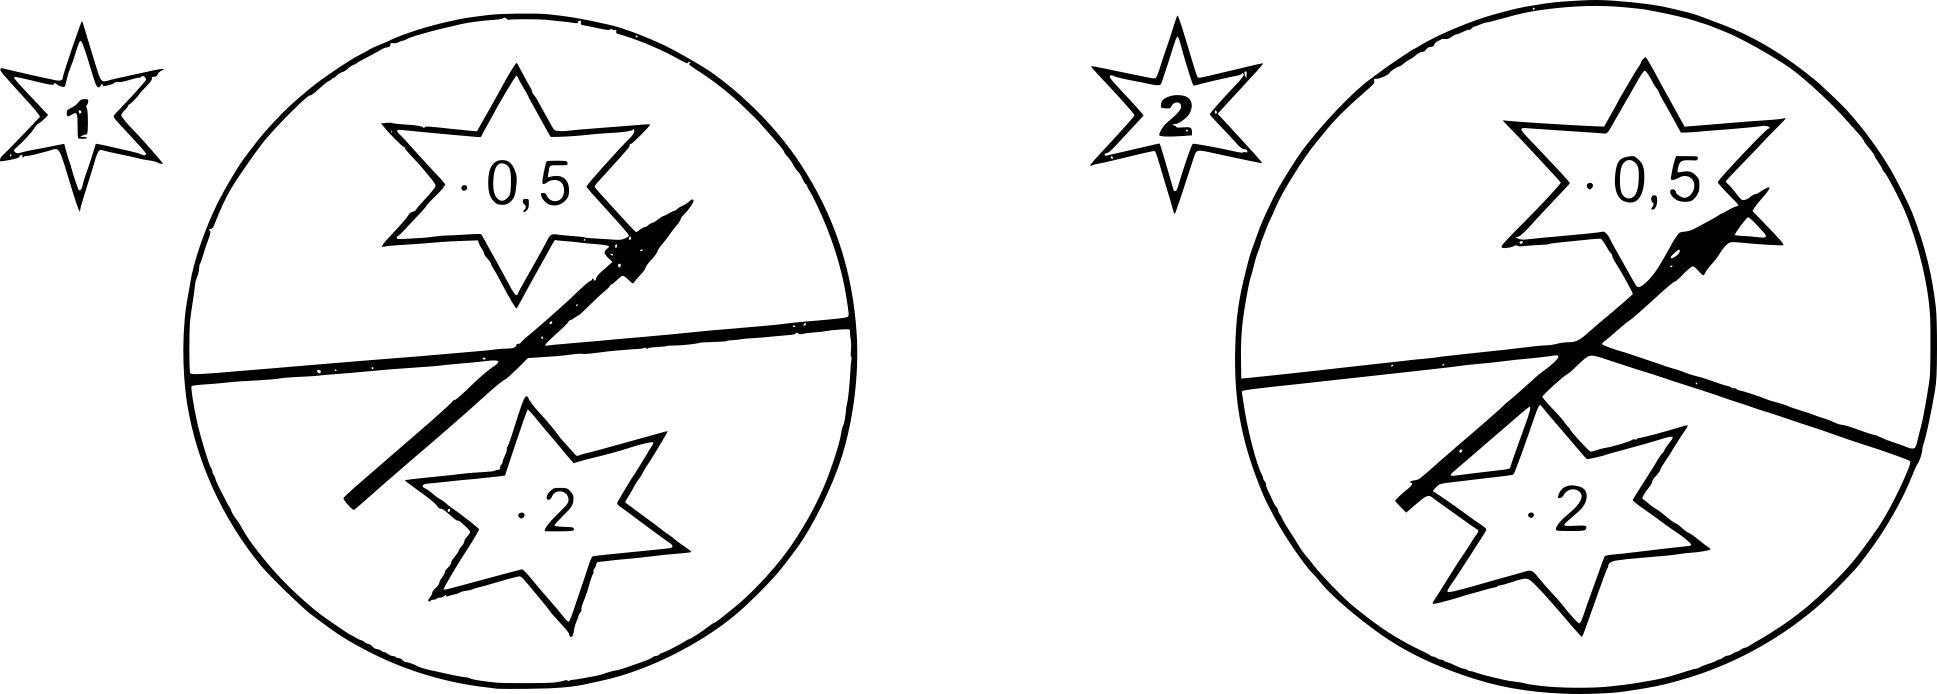
\includegraphics[width=0.7\columnwidth]{211203_gluecksraeder.png}
\end{figure}

\begin{enumerate}[label={\alph*)}] 
  \item Berechnen Sie den Erwartungswert für Ihren Gewinn, wenn das Glücksrad 1 benutzt wird.
  \item Berechnen Sie den Erwartungswert für Ihren Gewinn in Abhängigkeit von der Wahrscheinlichkeit $p$, mit der der Pfeil auf dem Feld $\cdot$2 stehen bleibt, wenn das Glücksrad 2 benutzt wird.
  \item Konstruieren Sie ein Glücksrad ähnlich wie das Glücksrad 2, sodass das Spiel als fair bezeichnet werden kann. Wie groß wird der Mittelpunktwinkel für das Feld $\cdot$2?
\end{enumerate}
%\vspace{2cm}



\end{document}
